\documentclass[
    article, 
    12pt, 
    oneside, 
    a4paper, 
    english, 
    brazil
    ]{abntex2}

\usepackage{lmodern}
\usepackage[T1]{fontenc}
\usepackage[utf8]{inputenc}
\usepackage{indentfirst}
\usepackage{nomencl}
\usepackage{color}
\usepackage{graphicx}
\usepackage{float}
\usepackage{tikz}
\usepackage{fourier}
\usepackage{microtype}
\usepackage{ragged2e}
\usepackage{lipsum}
\usepackage[brazilian,hyperpageref]{backref}
\usepackage[alf]{abntex2cite}

\setlength{\parindent}{1.3cm}
\setlength{\parskip}{0.2cm}
\SingleSpacing

\begin{document}

    \begin{tikzpicture}[remember picture, overlay]
        \node(Logo) at (current page.north west) [anchor=north west,xshift=2.5cm, yshift=-1.5cm] {
\includegraphics{img/logo.png}};
    \end{tikzpicture}

    \

    \begin{center}
        \textbf{REGÊNCIA E OBSERVAÇÃO DE TURMAS DE NÍVEL MÉDIO NO IFPI ZONA SUL}

        \
  
        \textbf{REGENCY AND OBSERVATION IN IFPI`S HIGH SCHOOL CLASSES}

        \

        \centering{Apresentação: Relato de Experiência}

        \

        João Victor dos Santos Mendes\footnote{Graduando de Licenciatura em Informática do Instituto Federal de Educação, Ciência e Tecnologia do Piauí, Campus Teresina Zona Sul. E-MAIL.}; Érika Lourrane Leôncio Lima\footnote{Professor/a Me. do Eixo de Disciplinas Pedagógica do curso de Licenciatura em Informática do Instituto Federal de Educação, Ciência e Tecnologia do Piauí, Campus Teresina Zona Sul. E-MAIL.}
    \end{center}

    \begin{OnehalfSpace}

    \noindent\textbf{INTRODUÇÃO}

    As salas de aula neste último século, estão mudando. Cada vez mais, a dinâmica entre professor e aluno, vêm se transformando devido ao avanço das tecnologias digitais. Celulares, tablets, redes sociais, vídeos online, bem como a capacidade de a poucos toques numa tela, ter acesso a basicamente qualquer informação têm mudado a dinâmica dos alunos nas salas de aula.
    
    Diante disso, um novo paradigma está surgindo no meio educacional, e o professor, terá um importante papel no ensino e interação com ela, utilizando-se de novas ferramentas e práticas pedagógicas disponíveis graças à essas tecnologias como intercâmbio de dados científicos e culturais, de diversa natureza, produção de texto em língua estrangeira, elaboração de jornais inter-escolas, permitindo o desenvolvimento de ambientes de aprendizagem centrados na atividade dos alunos, na importância da interação social, e no desenvolvimento de um espírito de colaboração e de autonomia nos alunos \cite{machado2002}.
    
    Este documento é um relato de experiência, trazendo informações acerca das atividades desenvolvidas e observações feitas em sala de aula pelo residente, bem como as atividades vivenciadas durante o cumprimento das etapas V e VI da residência pedagógica, realizadas nas datas que compreendem período que vai de setembro de 2019, à janeiro de 2020. 

\end{OnehalfSpace}
    \begin{OnehalfSpace}

    \noindent\textbf{RELATO DE EXPERIÊNCIA} 

    Os estágios aconteceram no Instituto Federal de Educação, Ciência e Tecnologia
    do Piauí (IFPI) Campus Zona Sul (IFPI-CTZS). Foram cumpridas 50h (cinquenta horas) de observação em quatro turmas diferentes no IFPI-CTZS da Segunda às Sexta-feiras no período da tarde e noturno. Na regência foram cumpridas 60h (sessenta horas) em uma turma, sendo nas Segunda-feira pela tarde. 
    
    Durante os dois estágios da residência, foi possível obter valiosas eperiências através de situações, tanto na regência, quanto na observação, situações essas que serão úteis para o futuro como um docente.

    Cada um dos professores observados tinha sua maneira de apresentar os mais diversos assuntos. Alguns deles expunham o conteúdo de forma expositiva, abrindo espaço no fim da explicação para que fosse tirado as dúvidas. Outros professores observados permitiam que os alunos ficassem mais à vontade no laboratório, permitindo que viessem tirar dúvidas enquanto praticavam nos computadores do laboratório. Nos dois casos, surgiam conversas paralelas, as quais os professores, com suas eperiências, conseguiam lidar com a situação, ainda mantendo os alunos à vontade. Os principais conteúdos abordados foram sobre a história e evolução dos computadores, \textit{Software} e \textit{Hardware} e história da \textit{Web}.

    Havia em uma das turmas de informática básica, um aluno surdo na sala, e era muito interessante acompanhar o desenvolvimento dele, bem como as experiências de ensino do docente. Os surdos possuem uma impossibilidade de ter uma memória sonora, e portanto, é necessário buscar alternativas de comunicação, segundo \cite{rinaldi1997} “devem basear-se na substituição da audição por outros canais, destacando-se a visão, o tato e movimento[...]”. Portanto a utilização de outros meios de comunicação, como a utilização mais ampla de imagens, e a prática de pesquisas \textit{online}, conseguiram melhorar o aproveitamento das mesmas.

    \begin{figure}[H]
        \centering
        \caption{Aula no laboratório de informática sobre Web.}
        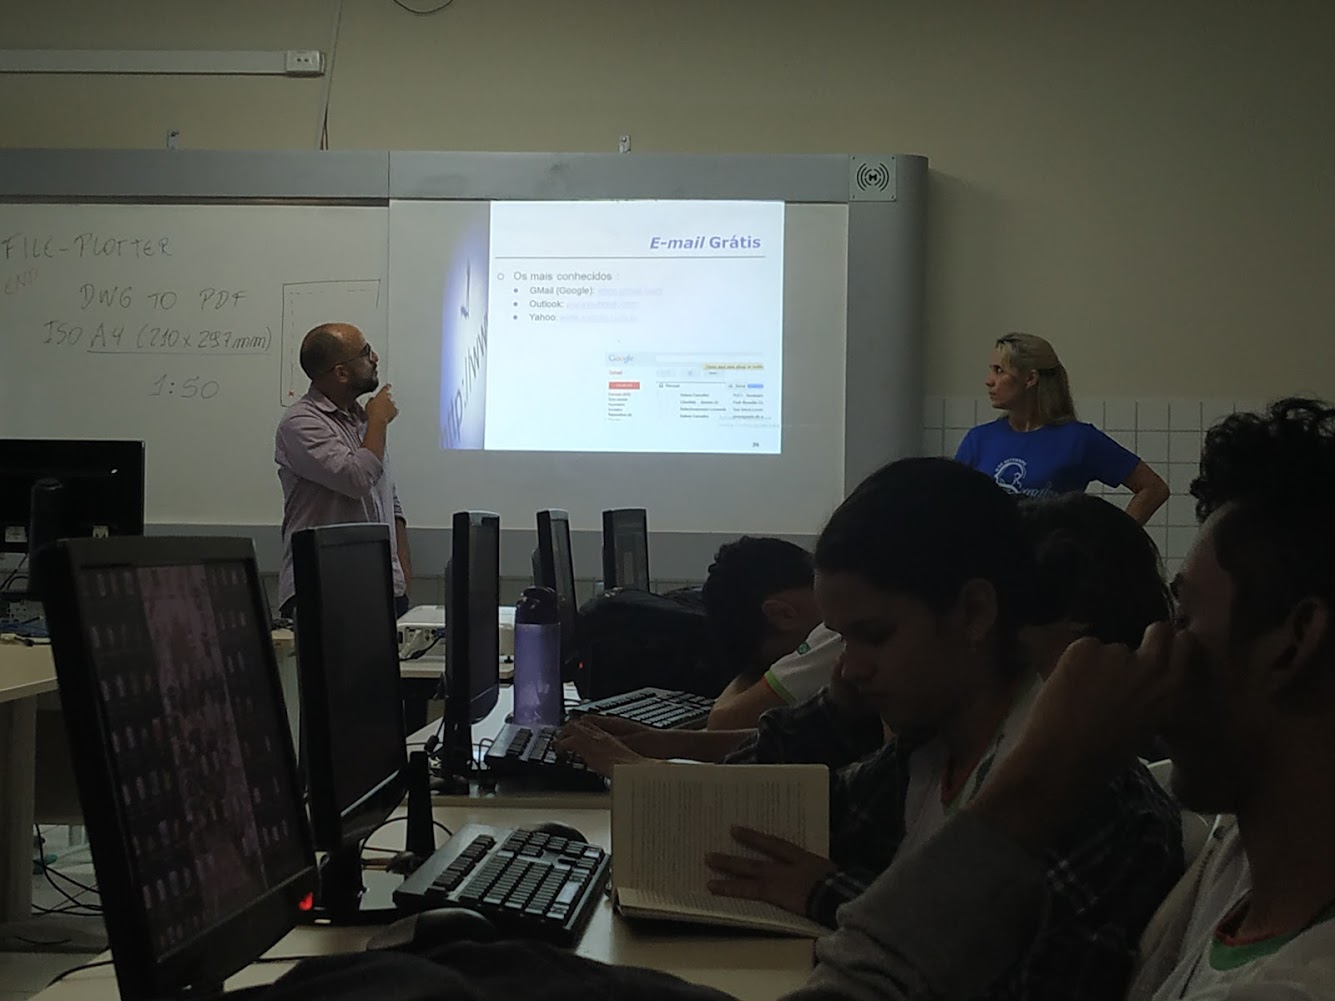
\includegraphics[width=100mm]{img/obs1-jef.jpg}
        \legend{Fonte: Própria}
        \label{figura}
    \end{figure}

    Durante a regência, foram abordados os conteúdos sobre história da computação, e em seguida, os programas do pacore \textit{Microsoft Office Word}, e \textit{Microsoft Office Excel}. Houve uma introdução à informática básica, antes de iniciar os trabalhos com as ferramentas do \textit{Office}, de forma a facilitar o aprendizado mais aprofundado dessas ferramentas. 
    A metodologia utilizada foi a expositiva dialogada.

    A regência trouxe consigo diversas novas experiências, que até então não tinham sido vivenciadas, onde foi possível acompanhar o desenvolvimento, e o processo de aprendizado dos alunos, desde o início do conteúdo, com toda a história da computação, até conceitos avançados de \textit{Excel}. 
    Desenvolver atividades, e provas, foi sem dúvida um grade desafio, visto que a quantidade de alunos na turma era maior que a quantidadede computadores que havia no laboratório, portanto as atividades, principalmente as avaliativas, deveriam ser planejadas para ser feita com os alunos em dupla ou sozinhos.

    Também foi notada uma dificuldade em alguns alunos, principalmente os que possuíam maior idade, com informática básica. Foi então, que foi dado um pequeno conteúdo sobre informática básica, ensinando conceitos de \textit{Windows}, como gerenciamento de pastas, gerenciamento de arquivos, área de trabalho, usuários, \textit{e-mail}, e arquivos em nuvem. Após este conteúdo, o ensino do pacote \textit{Office} ocorreu de forma mais natural.

    \begin{figure}[H]
        \centering
        \caption{Regência no laboratório de informática}
        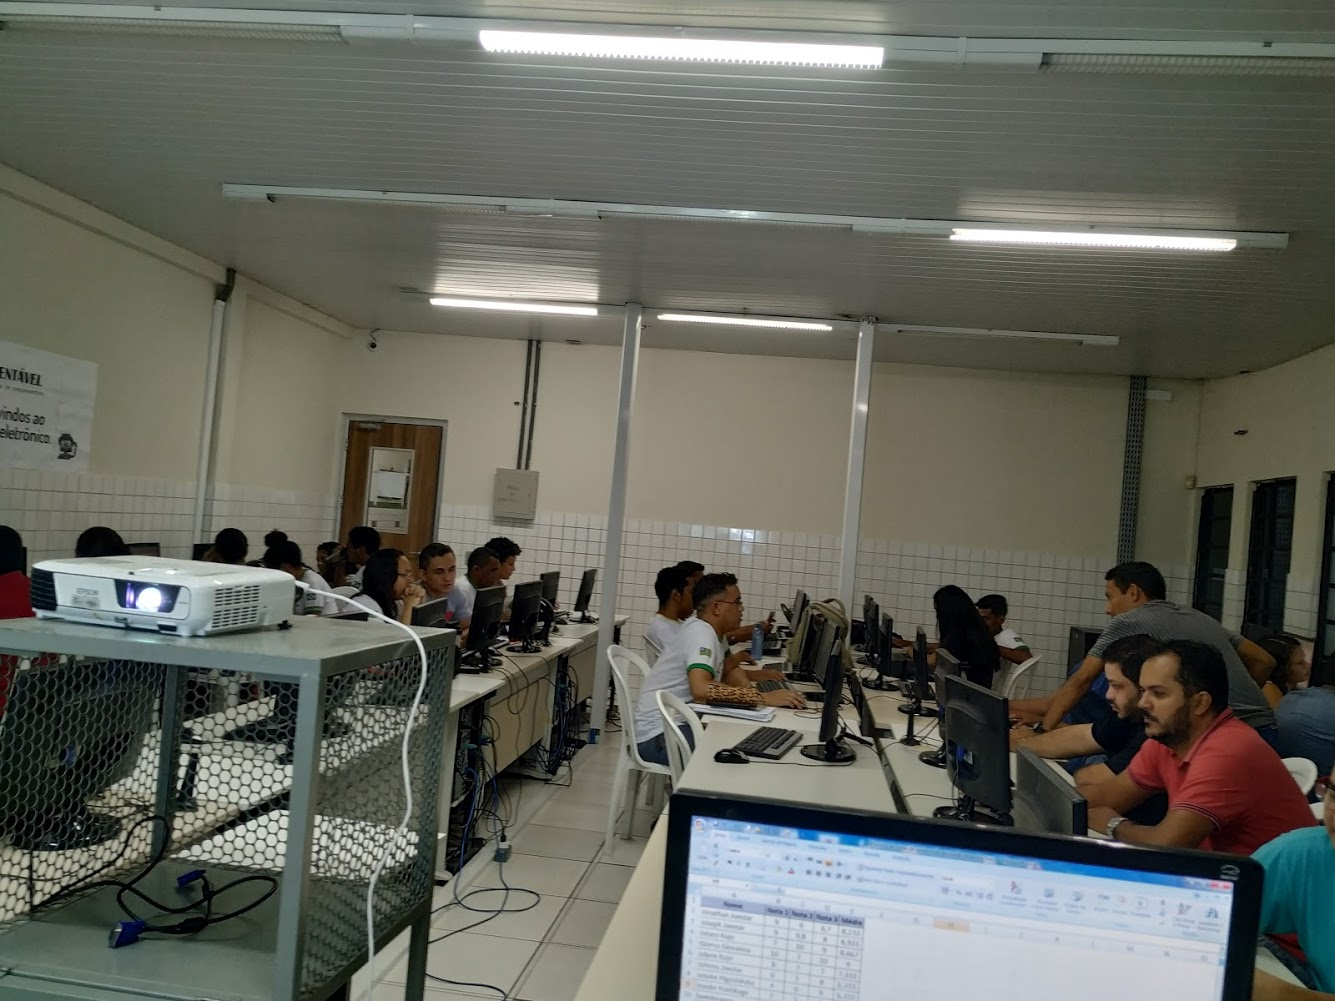
\includegraphics[width=100mm]{img/reg1.jpg}
        \legend{Fonte: Própria}
        \label{figura}
    \end{figure}


\end{OnehalfSpace}
    \begin{OnehalfSpace}
    \noindent\textbf{CONSIDERAÇÕES}

    São apresentadas as considerações sobre a experiência de extensão vivenciada, apontando possibilidades futuras de outras propostas. Neste momento são relacionadas às diversas ideias desenvolvidas ao longo do trabalho, num processo de síntese dos principais aspectos vivenciados, com os comentários do autor e as contribuições trazidas pela experiência.

\end{OnehalfSpace}
    \bibliography{referencias.bib}

\end{document}